\documentclass[main.tex]{subfiles}

\begin{document}

\defi{1}{.33}{Skalárpotenciálosság}

Egy $\rvec{v}: V \rightarrow V$ vektormező skalárpotenciálos,
ha $\exists \; \varphi : V \rightarrow \mathbb{R}$ skalármező,
hogy $\rvec{v} = \grad \; \varphi$.



\defi{1}{.33}{Vektorpotenciálosság}

Egy $\rvec{v}: V \rightarrow V$ vektormező vektorpotenciálos,
ha $\exists \; \rvec{u} : V \rightarrow V$ vektormező,
hogy $\rvec{v} = \rot \; \rvec{u}$.



\tetel{1}{.33}

$! \; \rvec{v}: V \rightarrow V$ mindenhol értelmezett,
legalább egyszer differenciálható vektormező, ekkor \dots
\begin{itemize}
  \item $\rvec{v}$ skalárpotenciálos $\Leftrightarrow$
        $\rot \; \rvec{v} = \rvec{0}$

  \item $\rvec{v}$ vektorpotenciálos $\Leftrightarrow$
        $\div \; \rvec{v} = 0$
\end{itemize}



\biz{0}{.50}{$\Rightarrow$ könnyű, $\Leftarrow$ nehéz}

Ha $\rvec{v}$ skalárpotenciálos, akkor
$\exists \; \varphi : V \rightarrow \mathbb{R}$,
hogy $\rvec{v} = \grad \; \varphi$, ekkor
$\rot \; \rvec{v} = \rot \; \grad \; \varphi \equiv \rvec{0}$
\\[.33em]
Ha $\rvec{v}$ vektorpotenciálos, akkor
$\exists \; \rvec{u} : V \rightarrow V$,
hogy $\rvec{v} = \rot \; \rvec{u}$, ekkor
$\div \; \rvec{v} = \div \; \rot \; \rvec{u} \equiv 0$



\azon{1}{.33}

$! \; \varPhi; \; \varPsi : \mathbb{R}^3
  \rightarrow \mathbb{R}$ skalármezők,
$\rvec{u}; \; \rvec{v}; \; \rvec{w} : \mathbb{R}^3
  \rightarrow \mathbb{R}^3$ vektormezők,
$\lambda; \mu \in \mathbb{R}$ skalárok.
\begin{itemize}
  \item Teljesül a linearitás:
        \begin{alignat*}{4}
          \grad & (\lambda \, \varPhi  &  & + \mu \, \varPsi)  &  & = \lambda \, \grad \, \varPhi &  & + \mu \, \grad \, \varPsi
          \\
          \rot  & (\lambda \, \rvec{v} &  & + \mu \, \rvec{w}) &  & = \lambda \, \rot \, \rvec{v} &  & + \mu \, \rot \, \rvec{w}
          \\
          \div  & (\lambda \, \rvec{v} &  & + \mu \, \rvec{w}) &  & = \lambda \, \div \, \rvec{v} &  & + \mu \, \div \, \rvec{w}
        \end{alignat*}

  \item Zérusság:
        \begin{alignat*}{1}
          \rot \, \grad \, \rvec{u} & \equiv \rvec{0}
          \\
          \div \, \rot \, \rvec{v}  & \equiv 0
        \end{alignat*}

  \item Deriválási szabályokhoz hasonló:
        \begin{align*}
          \grad \left( \varPhi \, \varPsi \right)
           & = \varPhi \, \grad \, \varPsi
          + \varPsi \, \grad \, \varPhi
          \\
          \div \left( \varPhi \, \rvec{v} \right)
           & = \varPhi \, \div \, \rvec{v} \,
          + \scalar{\rvec{v}}{\grad \, \varPhi}
          \\
          \rot \left( \varPhi \, \rvec{v} \right)
           & = \varPhi \, \rot \, \rvec{v}
          - \rvec{v} \cross \grad \, \varPhi
        \end{align*}

  \item Egyéb szabályok:
        \begin{align*}
          \rot \, \rot \, \rvec{v}
           & =\grad \, \div \, \rvec{v}
          - \Delta \rvec{v}
          \\
          \rot \left( \rvec{u} \cross \rvec{v} \right)
           & = \rvec{u} \, \div \, \rvec{v}
          - \rvec{v} \, \div \, \rvec{u}
          + (\Diff \rvec{u}) \rvec{v}
          - (\Diff \rvec{v}) \rvec{u}
          \\
          \div \left( \rvec{u} \cross \rvec{v} \right)
           & = \; \scalar{\rvec{v}}{\rot \, \rvec{u}}
          - \scalar{\rvec{u}}{\rot \, \rvec{v}}
          \\
          \grad \left( \scalar{\rvec{u}}{\rvec{v}} \right)
           & = (\Diff \rvec{u}) \rvec{v}
          + (\Diff \rvec{v}) \rvec{u}
          + \rvec{v} \cross \rot \, \rvec{u}
          + \rvec{u} \cross \rot \, \rvec{v}
        \end{align*}
\end{itemize}

\pagebreak
\biz{0}{0}{Azonosságok}
\pagebreak

%-------------------------------------------------------------------------------
%-------------------------------- Subsection 1.5 -------------------------------
%-------------------------------------------------------------------------------
\subsection{Vonalmenti integrál}

\defi{0}{.33}{Reguláris görbe}

Legyen $I \subset \mathbb{R}$ nem feltétlenül korlátos intervallum.
Ekkor az $\rvec{r} : I \rightarrow \mathbb{R}^3$ immerziót
reguláris görbének hívjuk.



\defi{1}{.33}{Pályasebesség}

A $\rvec{v} : I \rightarrow \mathbb{R}$,
$t \mapsto v(t) := \norma{\dot{\rvec{r}}(t)}$
függvényt pályasebességnek hívjuk.



\defi{1}{.33}{Ívhossz}

A pályasebesség $I$ feletti integrálját a
görbe ívhosszának nevezzük:
\begin{equation*}
  L(\rvec{r}) = \int_I \norma{\dot{\rvec{r}}(t)} \, \differential \, t
\end{equation*}



\defi{1}{.33}{Irányított görbe}

Egy $\rvec{r} : [ \, a; \, b \,] \rightarrow \mathbb{R}^3$ görbe
irányított, ha adott egy rendezés ($\leq$) a paraméterértékeken.
Ekkor $t_1 < t_2$ esetén $\rvec{r}(t_1)$ a görbe korábbi
pontja $\rvec{r}(t_2)$-höz képest. Ha $\rvec{r}(a) = \rvec{r}(b)$,
akkor a görbe zárt.



\megj{1}{0}{Irányítottság szemléltetése}

\begin{minipage}[c]{.49\textwidth}
  \begin{figure}[H]
    \centering
    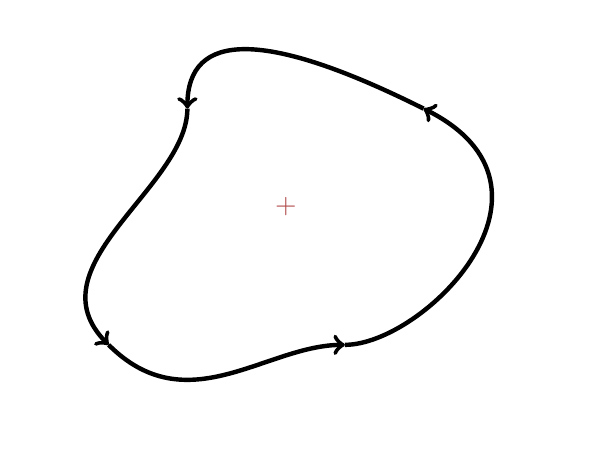
\begin{tikzpicture}
      \draw [ultra thick, <-] (0,0) .. controls (-1,1) and (1,2) .. (1,3);
      \draw [ultra thick, <-] (1,3) .. controls (1,4) and (2,4) .. (4,3);
      \draw [ultra thick, <-] (4,3) .. controls (6,2) and (4,0) .. (3,0);
      \draw [ultra thick, <-] (3,0) .. controls (2,0) and (1,-1) .. (0,0);


      \node[red!75!gray, thick, scale=3] at (2.25,1.75) {$\circlearrowleft$};
      \node[red!40!gray, thick, scale=1] at (2.25,1.75) {$+$};
    \end{tikzpicture}
    \caption{Pozitív irányítottságú görbe}
  \end{figure}
\end{minipage} \hfill
\begin{minipage}[c]{.49\textwidth}
  \begin{figure}[H]
    \centering
    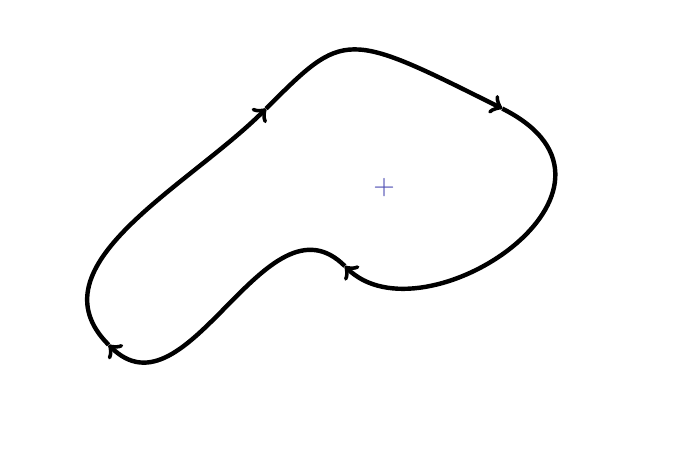
\begin{tikzpicture}
      \draw [ultra thick, ->] (0,0) .. controls (-1,1) and (1,2) .. (2,3);
      \draw [ultra thick, ->] (2,3) .. controls (3,4) and (3,4) .. (5,3);
      \draw [ultra thick, ->] (5,3) .. controls (7,2) and (4,0) .. (3,1);
      \draw [ultra thick, ->] (3,1) .. controls (2,2) and (1,-1) .. (0,0);

      \node[blue!75!gray, thick, scale=3] at (3.5,2) {$\circlearrowright$};
      \node[blue!40!gray, thick, scale=1] at (3.5,2) {$+$};
    \end{tikzpicture}
    \caption{Negatív irányítottságú görbe}
  \end{figure}
\end{minipage} \hfill


\allit{1}{.33}

He létezik a $\displaystyle \sum_ i \norma{
    \rvec{r}(t_i) - \rvec{r}(t_{i-1})
  }$ összeg sup\-remuma, akkor a görbe rektifikálható.
\begin{figure}[H]
  \centering
  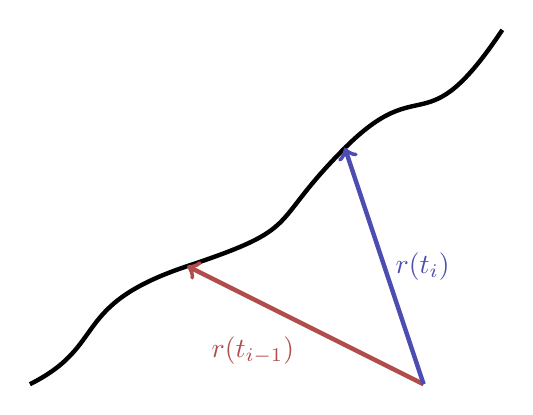
\begin{tikzpicture}
    \draw [ultra thick] (0, 0) .. controls (1, 0.5) and (0.5, 1) .. (2, 1.5);
    \draw [ultra thick] (2, 1.5) .. controls (3.5, 2) and (3, 2) .. (4, 3);
    \draw [ultra thick] (4, 3) .. controls (5, 4) and (5, 3) .. (6, 4.5);

    \draw [ultra thick, ->, red!40!gray]
    (5,0) -- (2,1.5)
    node [midway, below left] {$\rvec{r}(t_{i-1})$};

    \draw [ultra thick, ->, blue!40!gray]
    (5,0) -- (4,3)
    node [midway, right] {$\rvec{r}(t_{i})$};
  \end{tikzpicture}
  \caption{Görbe felnagyítva}
\end{figure}



\defi{1}{.33}{Vonalmenti integrál}

\begin{minipage}[c]{.4\textwidth}
  \begin{figure}[H]
    \centering
    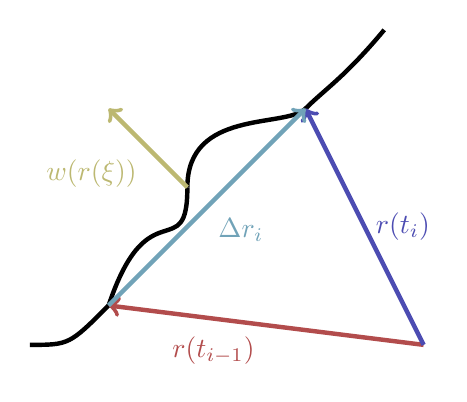
\begin{tikzpicture}
      \draw [ultra thick] (0, 0) .. controls (.5, 0) and (0.5, 0) .. (1, 0.5);
      \draw [ultra thick] (1, 0.5) .. controls (1.5, 2) and (2, 1) .. (2, 2);
      \draw [ultra thick] (2, 2) .. controls (2, 3) and (3.25, 2.75) .. (3.5, 3);
      \draw [ultra thick] (3.5, 3) .. controls (3.75, 3.25) and (4, 3.4) .. (4.5, 4);

      \draw [ultra thick, ->, red!40!gray]
      (5,0) -- (1,0.5)
      node [midway, below left] {$\rvec{r}(t_{i-1})$};

      \draw [ultra thick, ->, blue!40!gray]
      (5,0) -- (3.5,3)
      node [midway, right] {$\rvec{r}(t_{i})$};

      \draw [ultra thick, ->, cyan!40!gray]
      (1,0.5) -- (3.5,3)
      node [midway, below right] {$\Delta\rvec{r}_i$};

      \draw [ultra thick, ->, yellow!40!gray]
      (2, 2) -- (1,3)
      node [midway, below left] {$\rvec{w}(\rvec{r}(\xi))$};
    \end{tikzpicture}
    \caption{Görbe felnagyítva}
  \end{figure}
\end{minipage}
\begin{minipage}[c]{.58\textwidth}
  Ha a
  \begin{equation*}
    \displaystyle\sum_i \scalar{
      \rvec{w}(\rvec{r}(\xi))
    }{
      \rvec{r}(t_i) - \rvec{r}(t_{i-1})
    }
  \end{equation*}
  összegnek létezika a határértéke a görbe beosztásának
  minden határon túli finomítására nézve, akkor azt monjuk,
  hogy a $\rvec{w} : \mathbb{R}^3 \rightarrow \mathbb{R}^3$
  vektormező integrálható az $\rvec{r} : I \rightarrow \mathbb{R}^3$
  görbe mentén, és ezt a $\rvec{v}$ vektor $\rvec{r}$ görbe menti
  vonalintegráljának nevezzük. Jelölése:
  \begin{equation*}
    \int_{\rvec{r}} \scalar{\rvec{w}}{\differential \, \rvec{r}}
  \end{equation*}
\end{minipage}



\megj{1}{.33}

Belátható, hogy a görbe menti integrál létezéséhez elegendő,
hogy a vektormező csak a görbe mentén van értelmezve,
és ott szakaszonként folytonos.



\tetel{1}{.33}

Ha $\rvec{\gamma}$ egy görbe, melynek paraméteres egyenlete:
$\rvec{r} : I \rightarrow \mathbb{R}^3$, $t \mapsto \rvec{r}(t)$,
akkor a $\rvec{w}: \mathbb{R}^3 \rightarrow \mathbb{R}^3$ vektormező
$\rvec{\gamma}$ görbén vett (skalárértékű) integrálja:
\begin{equation*}
  \int_{\rvec{r}} \scalar{\rvec{w}}{\differential \, \rvec{r}}
  = \int_{t \in I} \scalar{
    \rvec{w}(\rvec{r}(t))
  }{\dot{\rvec{r}}(t)} \differential \, t
\end{equation*}



\biz{1}{0}

\begin{equation*}
  \scalar{
    \underbrace{\rvec{w}(\rvec{r}(\xi_i))}_{
      \rvec{w}(\rvec{r}(t))
    }
  }{
    \underbrace{\dfrac{
        \rvec{r}(t_i) - \rvec{r}(t_{i-1})
      }{t_i - t_{i-1}}}_{\dot{\rvec{r}}(t)}
  } (
  \underbrace{t_i - t_{i-1}}_{\differential t}
  )
\end{equation*}



\megj{1}{.33}

Ha a görbe irányítását megváltoztatjuk,
akkor az integrál értéke $(-1)$-szeresére változik.



\pelda{1}{0}
\pagebreak




\end{document}